\section{\textsc{ViTALBench} Dataset}
\label{sec:dataset}
\begin{figure*}[t]
\centering
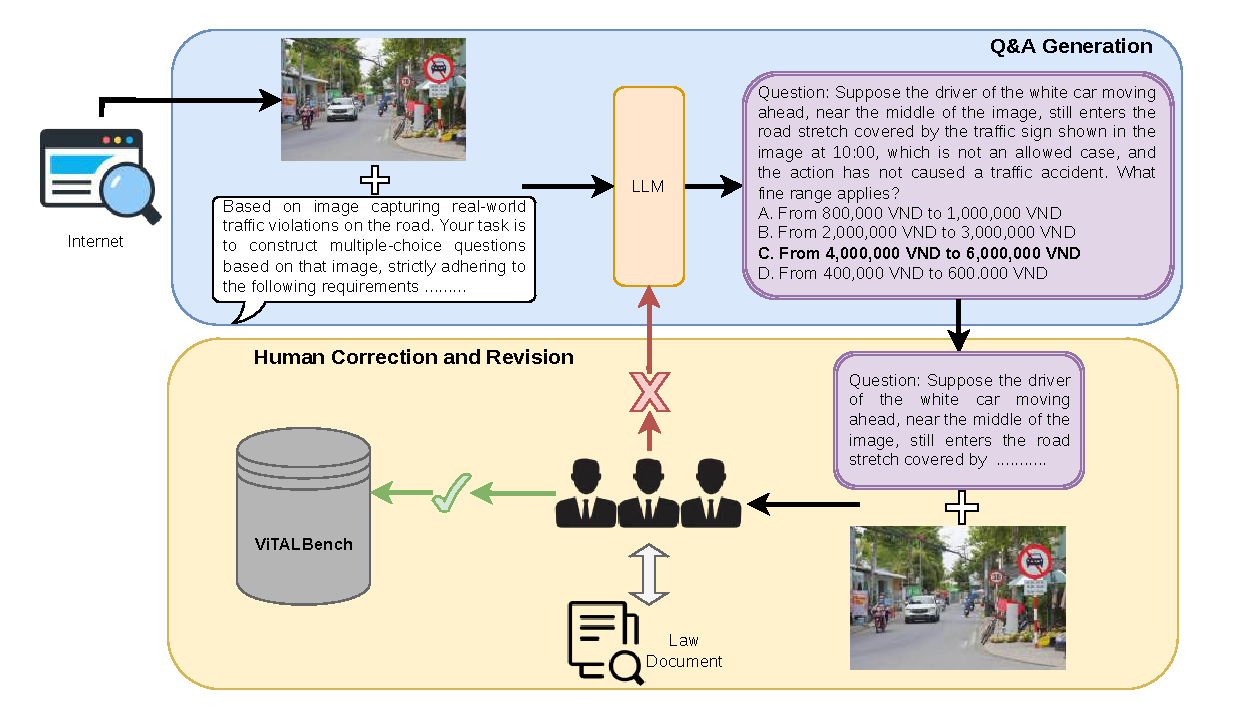
\includegraphics[width=0.9\textwidth]{Figures/Model.pdf}
\caption{Overview of the \textsc{ViTALBench} construction pipeline. Starting from real-world traffic images, an LLM generates candidate question-answer pairs and associated legal information, which are subsequently verified and refined by human annotators against official Vietnamese traffic regulations to produce the final benchmark.}
\label{fig:pipeline}
\end{figure*}

\textsc{ViTALBench} is constructed through a multi-stage pipeline that combines LLM-assisted annotation with human verification against official Vietnamese traffic regulations. As illustrated in Figure~\ref{fig:pipeline}, the pipeline consists of image collection, candidate question generation, manual verification, and benchmark curation.

\subsection{Dataset Construction}
\paragraph{Data collection.}
To ensure broad coverage, we first define a set of common violation categories based on current Vietnamese traffic regulations and search for images corresponding to each category. Images are collected from publicly accessible online sources, including news articles, traffic-safety websites, and publicly shared street photographs. Because traffic regulations vary across countries, \textsc{ViTALBench}  only focuses on scenarios governed by Vietnamese law. We retain only images that satisfy three criteria: \textbf{(1)} at least one traffic violation is visually identifiable; \textbf{(2)} the violation can be determined from a single frame, without temporal information; and \textbf{(3)} image quality is sufficient to recognize the relevant traffic participants and infrastructure. Duplicate and visually redundant images are removed during curation.

The resulting collection contains 551 images captured from diverse viewpoints, including street-level photographs and road cameras. It covers urban roads, intersections, residential streets, and highways, and includes motorcycles, passenger vehicles, buses, trucks, and pedestrians. All images are collected exclusively from publicly accessible sources for research purposes. Personally identifiable information, including visible faces and vehicle license plates, is anonymized or obscured when necessary to reduce privacy risks.

\paragraph{Legal knowledge base.}
We construct a legal knowledge base from three official documents governing road traffic in Vietnam. These include the National Technical Regulation on Road Signs and Signals, QCVN 41:2024/BGTVT, the Law on Road Traffic Order and Safety, Law No. 36/2024/QH15, and Decree No. 168/2024/ND-CP on administrative penalties for road traffic violations. Each document is segmented at the article level while preserving the document name, article identifier, and original legal text, resulting in 990 chunks. This organization allows annotators to retrieve and verify the provisions governing each observed violation and its corresponding legal consequences.

\paragraph{Hybrid human-AI annotation.}
Constructing legally grounded questions at scale requires both efficient generation and careful legal verification. LLMs can rapidly draft fluent questions and plausible distractors, but they may produce inaccurate citations or unsupported legal interpretations. Manual authoring alone, however, is costly and difficult to scale across thousands of questions and multiple legal documents. We therefore adopt a two-stage annotation protocol in which an LLM generates candidate instances and human annotators verify them against the legal knowledge base.
\paragraph{Stage 1. LLM drafting.}
GPT-5.5 is provided with the relevant legal context and used to generate initial instances for each image. Each draft contains a multiple-choice question, candidate answer options, the correct answer, the identified violation, and a reference to the potentially applicable legal provision. The model is instructed to produce distractors that are plausible within the traffic context but legally incorrect. All outputs are treated as preliminary drafts rather than final annotations.
\paragraph{Stage 2. Human verification against the legal corpus.}
Because a model may cite a provision that does not exist or does not apply, every draft is subsequently verified by a human annotator against the legal corpus. The annotator uses the identified violation and proposed citation as retrieval queries, reads the retrieved provisions, and checks three conditions. The identified violation must be fully supported by the visual evidence. The cited regulation must be legally accurate and applicable to the observed scenario. The question and answer options must be clear, legally unambiguous, and contain exactly one correct answer. When an instance fails any of these checks, the annotator provides the retrieved statutory evidence and revision instructions to the LLM. The revised instance is then verified again. This refinement process is limited to three rounds. Items that remain invalid or ambiguous after three rounds are removed. Samples are also discarded when they contain unsupported violations, incorrect legal references, or errors that cannot be reliably corrected.
\paragraph{Annotation quality assessment.}
To assess annotation reliability, we randomly sample 300 questions for independent human verification. Two experts knowledgeable in Vietnamese traffic regulations independently evaluate each question with respect to violation identification, statutory grounding, legal consequences, and answer correctness. The resulting agreement rate is $96.1\%$, with Cohen's $\kappa$ of $0.88$, indicating strong inter-annotator agreement. All disagreements are resolved through discussion before the final annotations are produced.

\paragraph{Reasoning Taxonomy}


Prior traffic VQA benchmarks distinguish between explicit scene perception and higher-level context-aware reasoning about traffic behavior and compliance. Building on this distinction, \textsc{ViTALBench} introduces a finer-grained taxonomy that decomposes legally grounded traffic reasoning into four categories with increasing dependence on statutory knowledge.


\begin{itemize}
    \item \textbf{Visual Perception.}
    These questions assess whether a model can recognize traffic-related elements directly observable in the image, including traffic signs, signals, lane markings, road layouts, vehicle types, participant positions, and visible behaviors. They require visual-semantic grounding but do not require a legal judgment.


    \item \textbf{Violation Identification.}
    These questions require the model to determine whether the observed behavior constitutes a traffic violation. Unlike visual perception, this category requires combining multiple scene cues, such as participant behavior, signal state, road structure, and surrounding context, to reach a compliance judgment. However, the model is not required to identify the specific governing provision or legal consequence.

    \item \textbf{Regulation Application.}
    These questions assume that the relevant behavior or violation has been identified and require the model to apply the corresponding statutory provision. The expected answer may concern the applicable fine, license-point deduction, license suspension, or another legal consequence. This category, therefore, evaluates whether a model can move from a recognized violation to a legally grounded decision.


    \item \textbf{Multi-step Legal Reasoning.}
    These questions require the complete reasoning process from visual evidence to legal consequence. A model must identify the relevant traffic participants and contextual cues, determine the violation, apply applicable legal conditions or exceptions, and select the final answer based on one or more statutory provisions. This category captures scenarios in which the legal conclusion depends on several interdependent visual and statutory conditions.

\end{itemize}



\subsection{Dataset Statistics}

\begin{figure*}[t]
\centering
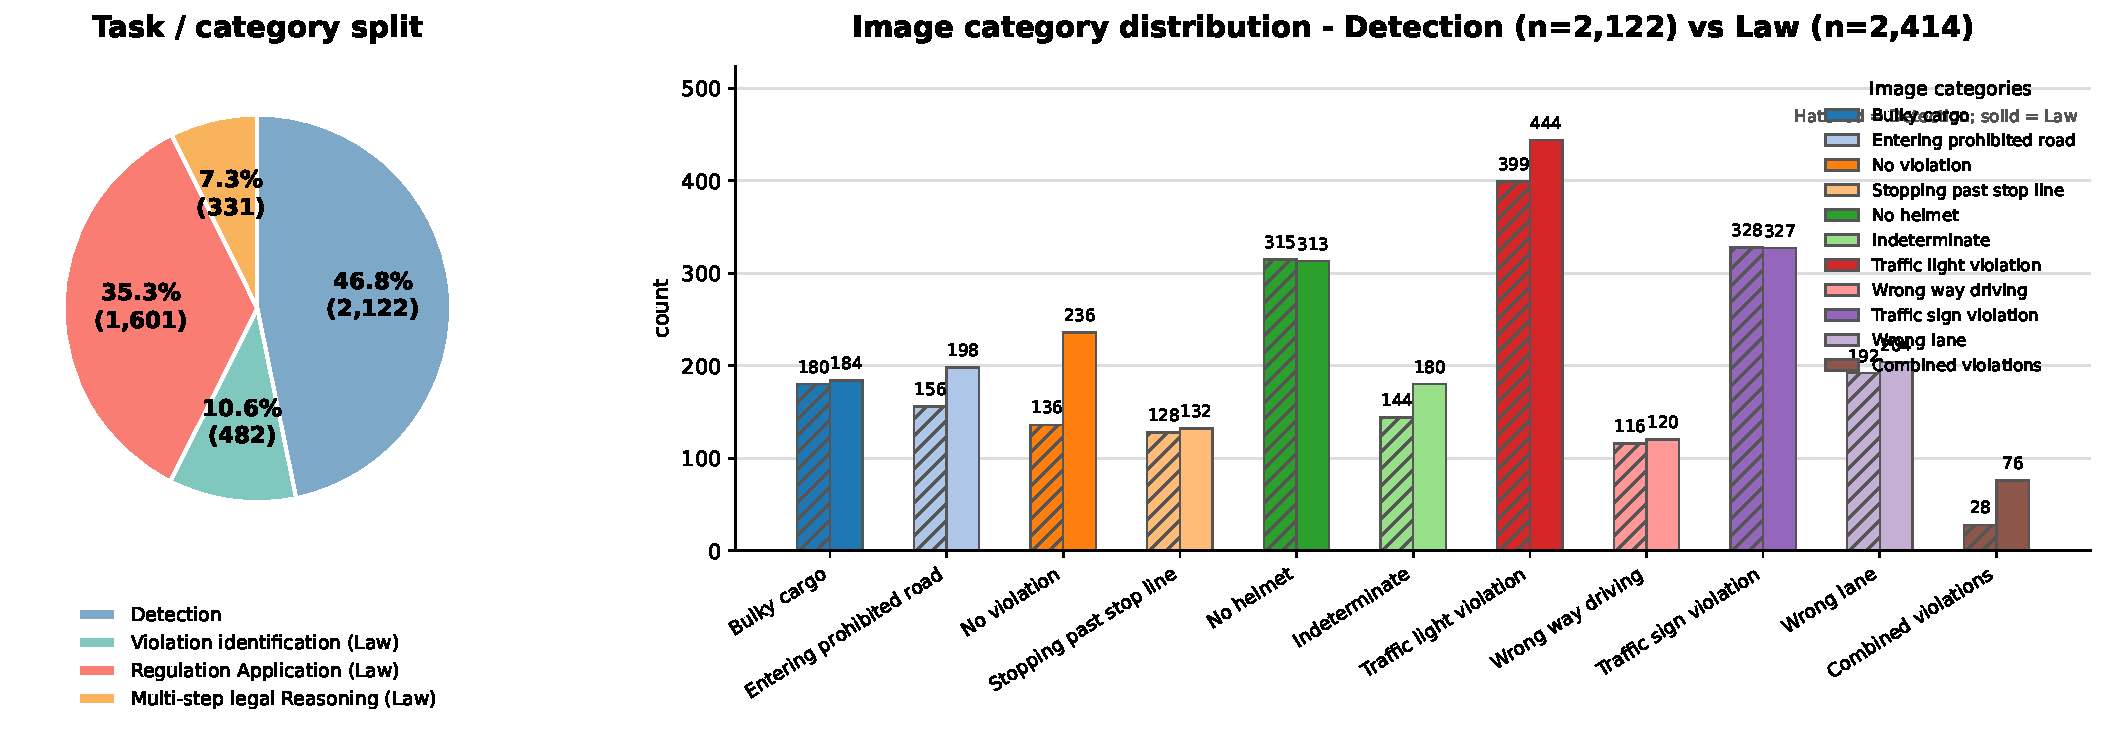
\includegraphics[width=\textwidth]{Figures/Statistic.pdf}
\caption{Statistics of \textsc{ViTALBench}.}
\label{fig:statistic}
\end{figure*}

Figure~\ref{fig:statistic} summarizes the statistics of \textsc{ViTALBench}. The release contains 4,536 multiple-choice questions over 551 images in 11 categories, including 2,122 detection questions and 2,414 law questions. The law questions comprise 482 Violation Identification questions, 1,601 Regulation Application questions, and 331 Multi-step Legal Reasoning questions. The accompanying release audit script computes these counts from the canonical files `detection.json`, `law.json`, `law_categories.json`, and `law_db.json`.

To reflect realistic traffic law enforcement scenarios, \textsc{ViTALBench} covers a broad spectrum of traffic violations rather than focusing on only a few frequently occurring cases. These include traffic-sign violations, lane usage, helmet regulations, speeding, illegal stopping and parking, wrong-way driving, vehicle loading, and other regulation-dependent behaviors. In addition, some benchmark instances contain multiple concurrent violations, requiring models to integrate multiple visual cues before determining the applicable regulation and legal consequence.

The reasoning-category distribution is intentionally imbalanced to better reflect the frequency and complexity of real-world traffic enforcement scenarios. Perception and Regulation Application account for approximately 80\% of the benchmark because these reasoning stages naturally arise in most traffic-law cases, whereas Multi-step Legal Reasoning represents comparatively rarer but substantially more complex scenarios. To mitigate the effects of this imbalance, we report both overall performance and category-wise accuracy in our experiments, enabling fair evaluation across different reasoning levels.